The runtime view is explained with the help of sequence diagrams, which shows the interaction between the components during runtime in a time flow depicting the order of which function takes place after another. The function names are same as the interface in order to help to relate the component, their interaction and their behavior during runtime. The sequence diagram of the three major services of TrackMe are shown which comprises the entire functioning of TrackMe and integrates to make the complete application.\newline
Here are the three sequence diagrams which briefly summarizes the runtime of the application.
\begin{figure}[H]
	\begin{center}
		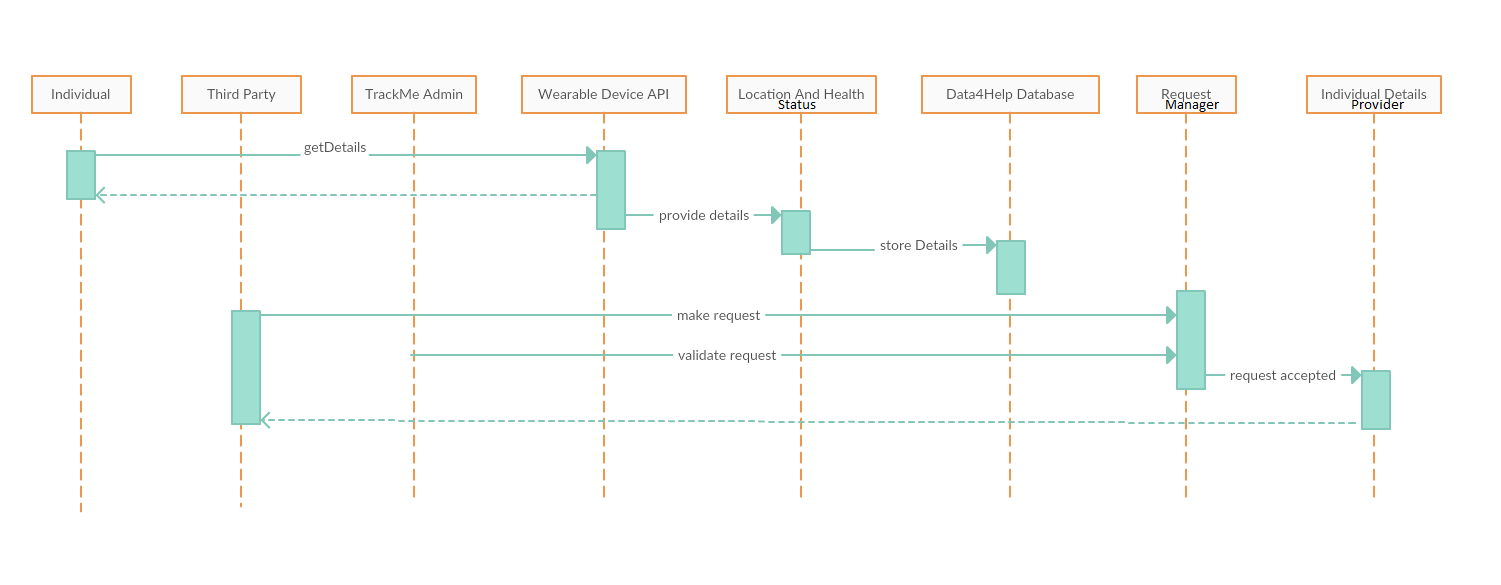
\includegraphics[width=\textwidth]{./DD_Diagrams/RuntimeData4Help.png}
      \caption{Sequence Diagram depicting runtime of Data4Help Service}
        \label{TrackMe_r1}
	\end{center}
\end{figure}
The location and health is taken from the user by the \textit{GetDetails Interface}  with the help of the API of the wearable device by \textit{ProvideDetails Interface}, which the individual selects from the list of compatible devices during registration. The details of the individual is then stored in the Data4Help database using \textit{StoreDetails Interface}.\newline
The thirdparty makes the request to access individual's data which is done by \textit{MakeRequest Interface}.\newline
The TrackMe Admin then validates the third party request and sends it to user to accept/reject or accepts/rejects himself according to the type of requests by \textit{ValidateRequest Interface}.\newline
If the request is accepted the user gets the access of the individual's details which uses the Data4Help Database in order to extract individual's details.
\begin{figure}[H]
	\begin{center}
		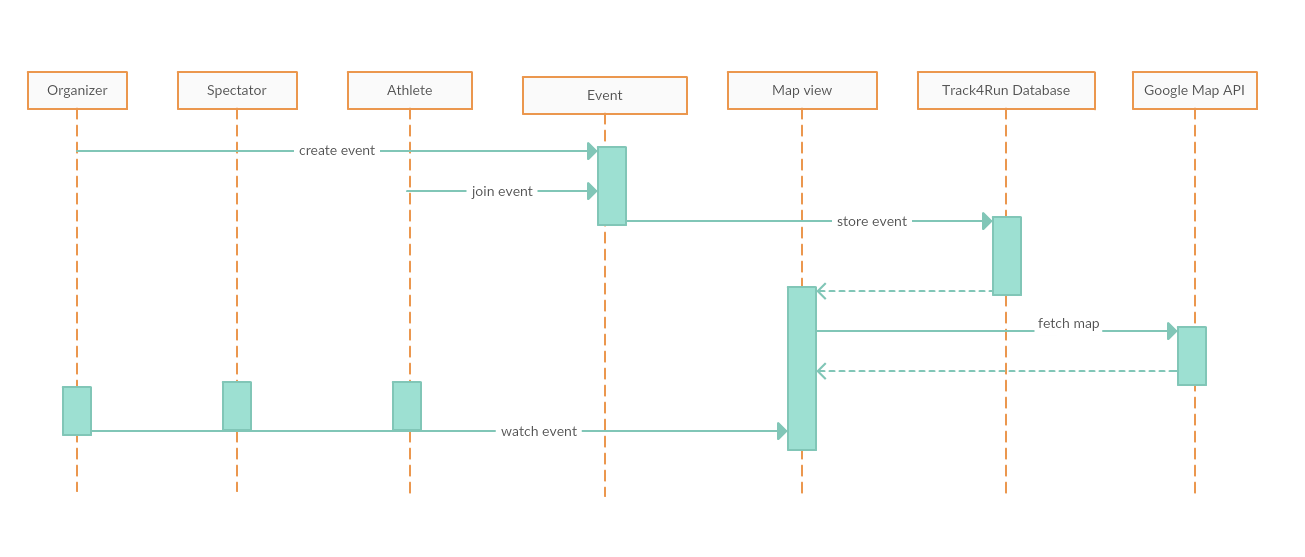
\includegraphics[width=\textwidth]{./DD_Diagrams/RuntimeAutomatedSOS.png}
      \caption{Sequence Diagram depicting runtime of AutomatedSOS Service}
        \label{TrackMe_r2}
	\end{center}
\end{figure}
Trackme checks the age of the user in order to know whether they are eligible for this service and checks the vitals to know about the emergency condition using  using \textit{CheckIndividualDetails Interface} which is fetched from the Data4Help Database and updated as Health Status component which contains the emergency vitals of individuals.\newline 
If the emergency situation is acknowledged the admin sends notification using \textit{SendPushNotification Interface} which includes the health status and location.\newline
The Individual receives the Ambulance Details by \textit{SendAmbulanceDetails Interface} and can track the ambulance whose information is fetched from the emergency Service API using \textit{FetchAmbulanceDetails Interface} and uses Maps API to show the map.
\begin{figure}[H]
	\begin{center}
		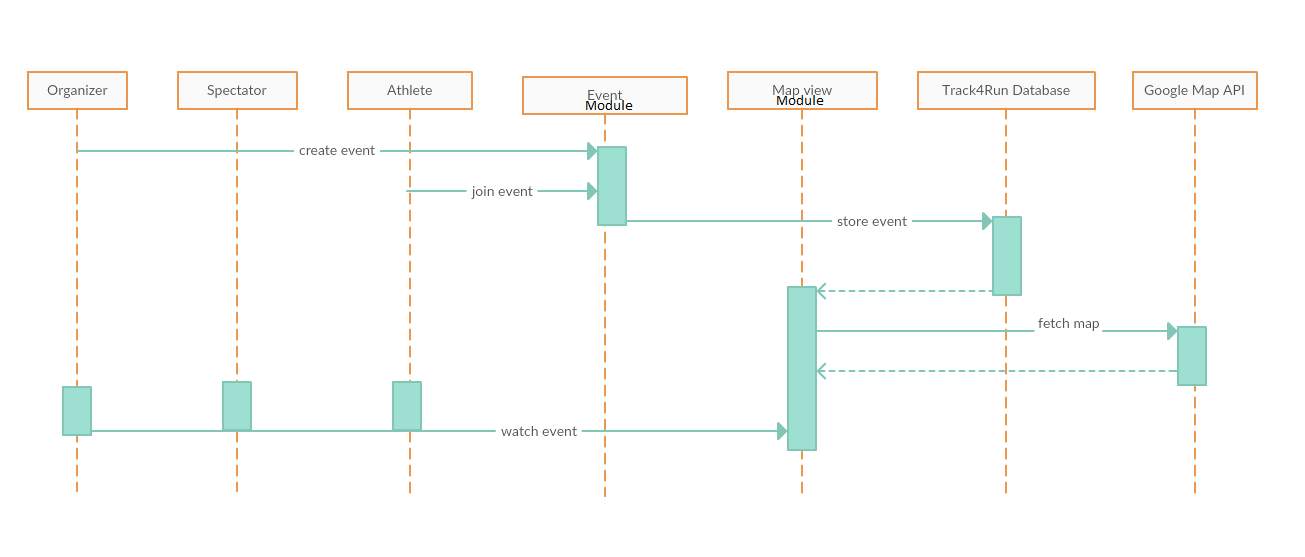
\includegraphics[width=\textwidth]{./DD_Diagrams/RuntimeTrack4Run.png}
      \caption{Sequence Diagram depicting runtime of Track4Run Service}
        \label{TrackMe_r3}
	\end{center}
\end{figure}
The organizer creates an event which the athlete joins using \textit{CreateEvent Interface} and \textit{JoinEvent Interface} respectively. The details of the event is store din the Track4Run Daatabase using \textit{StoreEvent Interface} which is used by Map view to show the details on map. The organizer, athlete and Spectator can watch the race in a map using \textit{WatchEvent Interface} which uses Map API to fetch the map.